% Being section ----------------------------------------------------------------
\section{Linear Algebra}

% Definitions subsection -------------------------------------------------------
\subsection{Definitions}

\begin{frame}{Matrices \& Vectors}

    Working with sums and multiplications of elements of matrices can get confusing very fast. Throughout the course, keep in mind the following representation for the outcome variable of interest:
    \begin{align*}
        Y_{n \times 1} = \begin{bmatrix} 
            y_1 \\
            y_2 \\
            \vdots \\
            y_n
            \end{bmatrix}
    \end{align*}

    So that scalar $y_i$ is the value for unit of observation $i$. This matrix holds information of the outcome variable of our sample with is of size $n$.
    
\end{frame}

\begin{frame}{Matrices \& Vectors}

    We will also use the following matrix to hold the values of our regressor variables:
    \begin{align*}
        X_{n \times k} = \begin{bmatrix} 
            x_{11} & x_{12} & \cdots & x_{1k} \\
            x_{21} & x_{22} & \cdots & x_{2k} \\
            \vdots & \vdots & \vdots & \vdots \\
            x_{n1} & x_{n2} & \cdots & x_{nk} \\
            \end{bmatrix}
    \end{align*}

    A column $k$ represents the value of variable $k$ for all $n$ units of observation. A row $i$ represents the value of all of our variables for unit of observation $i$. We will define the \textbf{transpose} of the $i$-th row of matrix $X$ as:
    \begin{align*}
        x_i = \begin{bmatrix} x_{i1} \\
                        x_{i2} \\ \cdots \\ x_{ik} \end{bmatrix}
    \end{align*}
    
\end{frame}

\begin{frame}{Matrix Operations as Summations}

    We can interpret a matrix operation using summations. For example (suppressing dimensionality subscript):
    \begin{align*}
        X' X &= \begin{bmatrix} 
                    x_{11} & x_{21} & \cdots & x_{n1} \\
                    x_{12} & x_{22} & \cdots & x_{n2} \\
                    \vdots & \vdots & \vdots & \vdots \\
                    x_{1k} & x_{2k} & \cdots & x_{nk} \\
                    \end{bmatrix}
                    \begin{bmatrix} 
                    x_{11} & x_{12} & \cdots & x_{1k} \\
                    x_{21} & x_{22} & \cdots & x_{2k} \\
                    \vdots & \vdots & \vdots & \vdots \\
                    x_{n1} & x_{n2} & \cdots & x_{nk} \\
                    \end{bmatrix}
        \\
        &= \begin{bmatrix} 
            x_1 & x_2 & \cdots & x_n
            \end{bmatrix}
            \begin{bmatrix} 
            x_1 \\ x_2 \\ \vdots \\ x_n
            \end{bmatrix}
        \\
        &= \sum_{i=1}^n x_i x_i'
    \end{align*}
    
\end{frame}

\begin{frame}{Matrix Operations as Summations}

    Given the definition of $Y$, we can also write:
    \begin{align*}
        X' Y = \begin{bmatrix} 
                x_1 & x_2 & \cdots & x_n
                \end{bmatrix}
                \begin{bmatrix} 
                y_1 \\ y_2 \\ \vdots \\ y_n
                \end{bmatrix} = \sum_{i=1}^n x_i y_i
    \end{align*}
    
    So, the OLS estimator can be written using summations as:
    \begin{align*}
        \hat{\beta}_{OLS} = (X' X)^{-1} X' Y = \Biggr( \sum_{i=1}^n x_i x_i' \Biggr)^{-1} \sum_{i=1}^n x_i y_i
    \end{align*}
    
\end{frame}


% Projections subsection -------------------------------------------------------
\subsection{Projections}

\begin{frame}{Projecting Vectors}

    A key concept to understand when dealing with linear regression is projection. Consider the following three-dimensional space representation.

    \begin{figure}[ht]
        \centering
        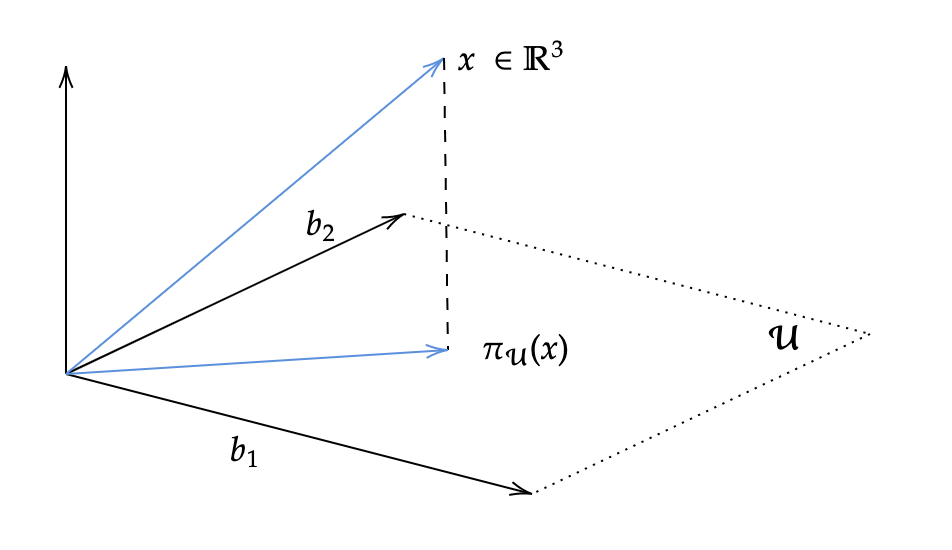
\includegraphics[width=0.5\linewidth]{./resources/projections.png}
    \end{figure}

    The vector $\pi_{\mathcal{U}}(x)$ is the orthogonal projection of vector $x$ onto space $\mathcal{U} = [ b_1, b_2 ]$, where $b_1$ and $b_2$ are the basis that span space $\mathcal{U}$.
    
\end{frame}

\begin{frame}{Projecting Vectors}

    We can represent $\pi_{\mathcal{U}}(x)$ as a linear combination of the basis vectors that span $\mathcal{U}$ since $\pi_{\mathcal{U}}(x) \in \mathcal{U}$.
    \begin{align*}
        \pi_{\mathcal{U}}(x) = \lambda_1 b_1 + \lambda_2 b_2
    \end{align*}

    Moreover, given that the difference vector $x - \pi_{\mathcal{U}}(x)$ is orthogonal to $\mathcal{U}$, its inner product with the basis vectors that span $\mathcal{U}$ must be zero.
    \begin{align*}
        \langle x - \pi_{\mathcal{U}}(x), b_1 \rangle &= 0
        \\
        \langle x - \pi_{\mathcal{U}}(x), b_2 \rangle &= 0
    \end{align*}

    This can be applied to an $M$-dimensional space.
    
\end{frame}

\begin{frame}{Generalizing to $M$-Dimensional Spaces}

    In an $M$-dimensional, define the following:
    \begin{align*}
        \lambda_{M \times 1} =  \begin{bmatrix}
                                    \lambda_1 \\
                                    \vdots \\
                                    \lambda_M \\
                                \end{bmatrix}, \quad
                                B_{D \times M} = \begin{bmatrix} b_1, \cdots, b_M \end{bmatrix}
    \end{align*}

    We can then write the equations we had in the previous slide as:
    \begin{align*}
        \pi_{\mathcal{U}}(x) &= \sum_{i=1}^M \lambda_i b_i
        \\
        \langle x - \pi_{\mathcal{U}}(x), b_i \rangle &= 0, \qquad i=1, \cdots, M
    \end{align*}

    where $x$ now is a $D$-dimensional vector. But as we saw before, we can write the first equation as:
    \begin{align*}
        \pi_{\mathcal{U}}(x) = \sum_{i=1}^M \lambda_i b_i = B \lambda
    \end{align*}
    
\end{frame}

\begin{frame}{Generalizing to $M$-Dimensional Spaces}

    Plug in the matrix representation to get:
    \begin{align*}
        \langle x - B \lambda, b_i \rangle &= 0
    \end{align*}

    The inner product satisfies the linearity property, which means that:
    \begin{align*}
        \langle x - B \lambda, b_i \rangle &= \langle x, b_i \rangle - \langle B \lambda, b_i \rangle= 0
    \end{align*}

    Applying the dot-product as an inner product space we get:
    \begin{align*}
        \langle x, b_i \rangle - \langle B \lambda, b_i \rangle &= 0
        \\
        x^T b_i - \lambda^T B^T b_i &= 0
    \end{align*}

    The last line above can be seen as a set of conditions for all basis $b_i$ in $i = 1, \cdots, M$, which allows us to write it as:
    \begin{align*}
        x^T B - \lambda^T B^T B &= 0_{M \times 1}
    \end{align*}
    
\end{frame}

\begin{frame}{Generalizing to $M$-Dimensional Spaces}

    Remember, we are interested in finding $\lambda$ that allows us to perform the orthogonal projection of an $M$-dimensional vector onto a $D$-dimensional space. We can re-arrange the above and play around with it:
    \begin{align*}
        x^T B - \lambda^T B^T B &= 0_{M \times 1}
        \\
        \lambda^T B^T B &= x^T B
        \\
        \lambda^T &= x^T B (B^T B)^{-1}
        \\
        \lambda &= (B^T B)^{-1} B^T x
    \end{align*}

    where above we use the fact that $(B^T B)^{-1} = [(B^T B)^{-1}]^T$ since $(B^T B)^{-1}$ is a symmetric matrix, so its inverse equals the original matrix. \textbf{Does this look familiar?}
    
\end{frame}

\begin{frame}{Generalizing to $M$-Dimensional Spaces}

    To recap, we said that:
    \begin{align*}
        \pi_{\mathcal{U}}(x) &= B \lambda
        \\
        \lambda &= (B^T B)^{-1} B^T x
    \end{align*}

    Combine the two equations and we have that:
    \begin{align*}
        \pi_{\mathcal{U}}(x) &= \underbrace{B (B^T B)^{-1} B^T}_{\text{projection matrix}} x
    \end{align*}

    So the matrix $B (B^T B)^{-1} B^T$ projects the $M$-dimensional vector $x$ onto the $D$-dimensional space spanned by the basis vectors in $B$.
    
\end{frame}